% !TeX root = ../main.tex
% Add the above to each chapter to make compiling the PDF easier in some editors.
\chapter{Artificial Neural Networks}\label{chapter:Related Work}
Artificial Neural Networks, or simply Neural Networks, are certain kind of computing systems that are inspired by the functionality of Biological Neural Networks, for Example the brains of mammals'. ANNs are import representatives or techniques for modern Artificial Intelligence, although the idea of NNs is not as new as the recent hype over them, seen in the last couple years. Actually, the beginning of ANNs point back to the 1940s. These networks are basically trained by feeding data and telling them what the corresponding output should look like. So what has changed over the last couple of years, is the massive amount of new data and a general increase in computing power, these two major advantages over earlier years, may have been contributed to the new success of Artificial Neural Networks.

\section{Fundamentals}

\begin{figure}[H]
	\centering
	\minipage{0.47\textwidth}
	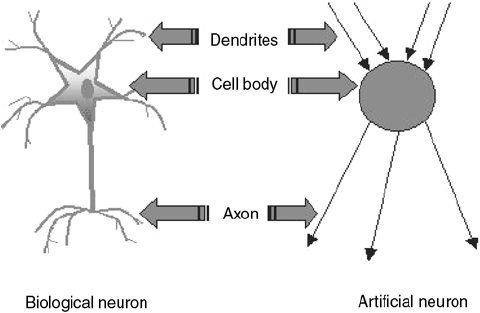
\includegraphics[width=\linewidth]{images/Fig-1-Analogy-between-artificial-neuron-and-biological-neuron.png}
	\caption{Biological and Artificial Neuron}
	\label{fig:artifical_and_biological}
	\endminipage\hfill
	\minipage{0.4\textwidth}
	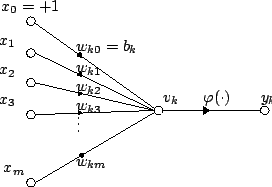
\includegraphics[width=\linewidth]{images/artificial_neuron.png}
	\caption{Single Artificial Neuron}
	\label{fig:artificial_neuron}
	\endminipage
\end{figure}

\subsection{Neurons}
As already mentioned, ANNs have several things in common with Biological Neural Networks, in this Analogy, an Artificial Neuron is a simplified abstraction of a Biological Neuron, both have a cell body and incoming respectively outgoing connections, called Dendrites and Axons (Figure: \ref{fig:artifical_and_biological}). Every arriving signal over the Dendrite is first multiplied with it's corresponding weight, then added together. Be noted that $x_{0}$ is no input signal from a different Neuron, but rather is always set to 1 and is called the bias input. \newline
After totalizing the input values, our signal is channeled through an activation- or transfer function (Figure \ref{fig:artificial_neuron}). There are several possibilities for the transformation function to choose from, which aims to handle when the Neuron produces output and when it remains silent. Another reason would be to keep the values between certain boundaries, usually it is desirable to stay in range [0;1]. Common transfer functions would be the Sigmoid- (\ref{eqn:sigmoid}) and the Heaviside Step Function (\ref{eqn:heaviside}). Coming back to previous analogy, the Sum-Operator in series connection to the Activation function form the artificial cell body.\newline 
After forming an output signal $y_{k}$ (\ref{eqn:dendrites_sum}), the Axon can fork into one or multiple branches, serving one or multiple Neurons as it's or their input dendrites, after they have been weighted by their corresponding new weights.   


\begin{equation}
\label{eqn:vk}
	v_{k} = \sum_{i=0}^{m} x_{i} w_{ki}
\end{equation}  

\begin{equation}
	\label{eqn:dendrites_sum}
	y_{k} = \varphi(v_{k}) = \varphi(\sum_{i=0}^{m} x_{i} w_{ki}) 
\end{equation} 

\begin{equation}
	\label{eqn:sigmoid}
	S(x) = \frac{e^x}{e^x + 1} = \frac{1}{1 + e^{-x}}
\end{equation} 

\begin{equation}
	\label{eqn:heaviside}
	H(x)= 
	\begin{cases}
	1,& x\geq 0\\
	0,& x < 0
	\end{cases}
\end{equation}

\subsection{From Neurons To Networks}


\section{Common Types}
